%Kurzfassung

Die Modularisierungskonzepte für die Prozessindustrie erhöhen die Flexibilität. Der Anlagenbediener wird dabei vor die Herausforderung gestellt, Probleme nicht mehr auf Grundlage von umfangreicher Erfahrung lösen zu können. Assistenzsysteme können dem Menschen mittlerweile viele Aufgaben abnehmen und ihn somit bei einem Problemlöseprozess begleiten. Die Analyse dieser Arbeit zeigt die Vielschichtigkeit der Einflussfaktoren auf Problem und Lösung auf. Damit der Nutzer dennoch jederzeit einen Überblick behält, wird er durch die entwickelte Interaktionsplattform unterstützt. Diese lenkt die Aufmerksamkeit auf die relevanten Informationen. Unter Experten findet die Einfachheit des Systems und die Übersichtlichkeit der Lösungen sehr positiven Anklang und würde von diesen auch empfohlen werden.

\vspace{10pt}
\begin{center}
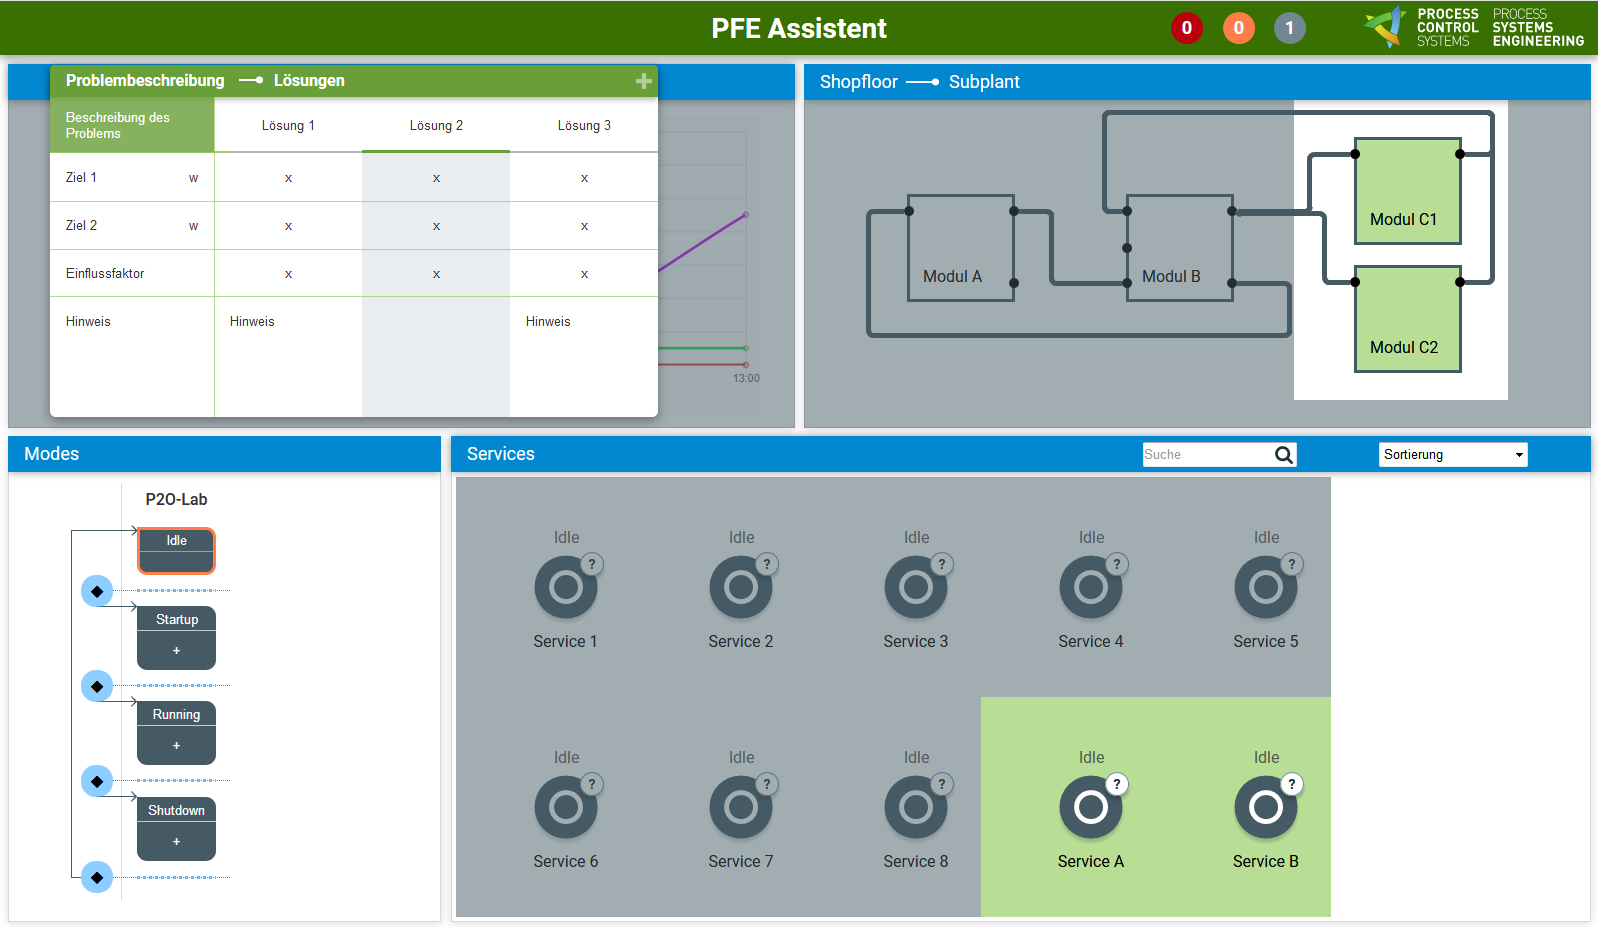
\includegraphics[scale=0.25]{DA_files/Bilder/Konzept/Skizze-Loesungen-PFE.png}
%[keepaspectratio, width=13 cm]
\end{center}
\vspace{6pt}